\section{eo\-Sequential\-Op$<$ EOT $>$ Class Template Reference}
\label{classeo_sequential_op}\index{eoSequentialOp@{eoSequentialOp}}
Sequential selection: note the mark, rewind, unmark cycle here operators are repeatedly applied on the same individual(s) not all too elegant, but it sort of works...  


{\tt \#include $<$eo\-Op\-Container.h$>$}

Inheritance diagram for eo\-Sequential\-Op$<$ EOT $>$::\begin{figure}[H]
\begin{center}
\leavevmode
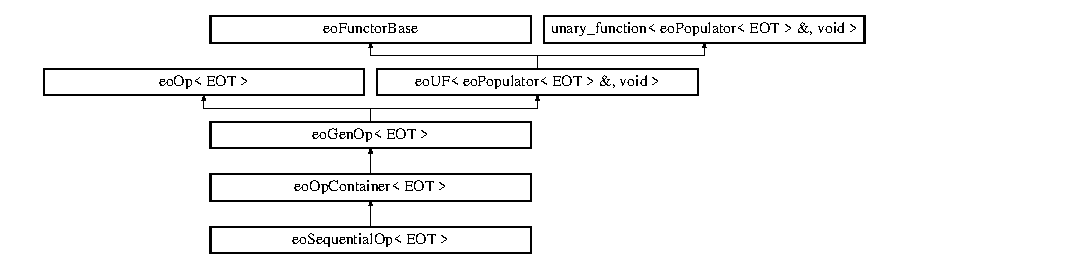
\includegraphics[height=3.18544cm]{classeo_sequential_op}
\end{center}
\end{figure}
\subsection*{Public Types}
\begin{CompactItemize}
\item 
typedef unsigned {\bf position\_\-type}\label{classeo_sequential_op_w0}

\end{CompactItemize}
\subsection*{Public Member Functions}
\begin{CompactItemize}
\item 
void {\bf apply} ({\bf eo\-Populator}$<$ {\bf EOT} $>$ \&\_\-pop)\label{classeo_sequential_op_a0}

\begin{CompactList}\small\item\em the function that will do the work \item\end{CompactList}\item 
virtual std::string {\bf class\-Name} () const \label{classeo_sequential_op_a1}

\end{CompactItemize}
\subsection*{Private Attributes}
\begin{CompactItemize}
\item 
std::vector$<$ size\_\-t $>$ {\bf to\_\-apply}\label{classeo_sequential_op_r0}

\item 
std::vector$<$ size\_\-t $>$ {\bf production}\label{classeo_sequential_op_r1}

\end{CompactItemize}


\subsection{Detailed Description}
\subsubsection*{template$<$class EOT$>$ class eo\-Sequential\-Op$<$ EOT $>$}

Sequential selection: note the mark, rewind, unmark cycle here operators are repeatedly applied on the same individual(s) not all too elegant, but it sort of works... 



Definition at line 88 of file eo\-Op\-Container.h.

The documentation for this class was generated from the following file:\begin{CompactItemize}
\item 
eo\-Op\-Container.h\end{CompactItemize}
